\documentclass[
	% -- opções da classe memoir --
	12pt,				% tamanho da fonte
	openright,			% capítulos começam em pág ímpar (insere página vazia caso preciso)
	oneside,			% para impressão em um lado. Oposto a twoside, verso e anverso
	a4paper,			% tamanho do papel. 
	% -- opções da classe abntex2 --
	chapter=TITLE,		% títulos de capítulos convertidos em letras maiúsculas
	section=TITLE,		% títulos de seções convertidos em letras maiúsculas
	%subsection=TITLE,	% títulos de subseções convertidos em letras maiúsculas
	%subsubsection=TITLE,% títulos de subsubseções convertidos em letras maiúsculas
	% -- opções do pacote babel --
	english,			% idioma adicional para hifenização
	%french,			% idioma adicional para hifenização
	%spanish,			% idioma adicional para hifenização
	brazilian,			% o último idioma é o principal do documento
	]{styles/abntex2}

\usepackage[alf,
%versalete,
abnt-emphasize = bf, % destaca o titulo da revista ou livro em negrito;
abnt-etal-list = 3, % trabalhos com mais de 3 autores recebem et al.,;
%abnt-etal-text = it, % escreve o et al., em italico;
%abnt-and-type = e, % usa o caracter '&' no lugar de 'e' para mais de um autor;
abnt-last-names = abnt, % trata sobrenomes 'estritamente' conforme a ABNT;
abnt-repeated-author-omit = no % autores com + de uma entrada recebem '____.'
]{styles/abntex2cite}

\usepackage[utf8]{inputenc}

%\usepackage[dvipsnames]{xcolor}
\usepackage[table,xcdraw,dvipsnames]{xcolor}
%\usepackage{subfigure}   % Pacote para subfiguras
\usepackage{amsmath}
\usepackage{lastpage}
\usepackage{times}
\usepackage{graphicx}
\usepackage{caption}
\usepackage{tocloft}
\usepackage{tabularx}
\usepackage{booktabs}
\usepackage{enumitem}
\usepackage{dirtytalk}
\usepackage{tikz}
\usetikzlibrary{tikzmark}
%\usepackage{array} 
\usepackage{multirow}
\usepackage{threeparttable} % to use table notes

\usepackage{caption}
\usepackage{textcomp}


%%%%%%%%%%%%%%%%%%%%%%%%%%%%%%%%%%%%%%%%%%%%%%%%%%%%%%%%%%%%%%%%%
%%%%%%%%%%%%%%%%%%%%%%%%%%%%%%%%%%%%%%%%%%%%%%%%%%%%%%%%%%%%%%%%%
%%%%%%%%%%%%%%%%%%%%%%%%%%%%%%%%%%%%%%%%%%%%%%%%%%%%%%%%%%%%%%%%%
\usepackage{listings}
\usepackage{xcolor}

%New colors defined below
\definecolor{codegreen}{rgb}{0,0.6,0}
\definecolor{codegray}{rgb}{0.5,0.5,0.5}
\definecolor{codepurple}{rgb}{0.58,0,0.82}
\definecolor{backcolour}{rgb}{0.95,0.95,0.92}

%Code listing style named "mystyle"
\lstdefinestyle{mystyle}{
  backgroundcolor=\color{backcolour}, commentstyle=\color{codegreen},
  keywordstyle=\color{magenta},
  numberstyle=\tiny\color{codegray},
  stringstyle=\color{codepurple},
  basicstyle=\ttfamily\footnotesize,
  breakatwhitespace=false,         
  breaklines=true,                 
  captionpos=b,                    
  keepspaces=true,                 
  numbers=left,                    
  numbersep=5pt,                  
  showspaces=false,                
  showstringspaces=false,
  showtabs=false,                  
  tabsize=2
}

%"mystyle" code listing set
\lstset{style=mystyle}
%%%%%%%%%%%%%%%%%%%%%%%%%%%%%%%%%%%%%%%%%%%%%%%%%%%%%%%%%%%%%%%%%
%%%%%%%%%%%%%%%%%%%%%%%%%%%%%%%%%%%%%%%%%%%%%%%%%%%%%%%%%%%%%%%%%
%%%%%%%%%%%%%%%%%%%%%%%%%%%%%%%%%%%%%%%%%%%%%%%%%%%%%%%%%%%%%%%%%


% Criação do symbol da função sign
\DeclareMathOperator{\sign}{sign}

\newcolumntype{C}[1]{>{\centering\let\newline\\\arraybackslash\hspace{0pt}}m{#1}}
\newcolumntype{L}[1]{>{\RaggedRight\let\newline\\\arraybackslash\hspace{0pt}}m{#1}}

% Alinhamento de legenda à esquerda
\captionsetup{justification=raggedright,singlelinecheck=false}

\usepackage{styles/ttc_univali}

\begin{document}
\newcounter{equationCounter}

\pretextual

\begin{Info}
% Universidade
{UNIVERSIDADE DO VALE DO ITAJAÍ}
% Escola
{ESCOLA POLITÉCNICA}
% Curso
{CURSO DE CIÊNCIA DA COMPUTAÇÃO}
% Titulo
{DETECÇÃO DE ERROS EM SISTEMA OPERACIONAL DE TEMPO REAL}
% Autor
{Marcos Augusto Fehlauer Pereira}
% Cidade e Data
{Itajaí (SC), Junho de 2025}
% Nome da Área de concentração
{Sistemas Operacionais}
% Orientador(a)
{Felipe Viel, MSc.}
% Coorientador(a) <Nome do Coorientador(a)>, <Titulação> %%%%%%%% Se não tiver coorientador deixe vazio

\end{Info}

%\begin{Dedicatoria}
% Dedicatória
% \end{Dedicatoria}

% \begin{Agradecimentos}
% Agradeço a todos.
% \end{Agradecimentos}

% \begin{Epigrafe}
% Epígrafe
% \end{Epigrafe}

\begin{Resumo}
Sistemas embarcados são sistemas especializados tipicamente encontrados como um componente lógico de um dispositivo maior, estes sistemas utilizam-se com frequência um tipo especializado de sistema operacional: Sistemas operacionais de tempo real, que permitem que múltiplas tarefas executem de forma concorrente. Em diversas situações é necessário que esses dispositivos operem em condições adversas (como radiação ionizante e interferência eletromagnética) que alteram seu comportamento esperado e degradam sua qualidade de serviço, para operar dentro de tais condições, técnicas de tolerância à falhas são aplicadas, que visam permitir a operação razoável do sistema mesmo na presença de falhas. Para viabilizar tolerância à falhas é possível utilizar de diversos mecanismos, dentre eles, aqueles que operam em conjunto com o escalonador do sistema operacional de tempo real podem permitir um grau de resiliência maior enquanto visando reduzir a ociosidade dos núcleos da máquina. Este trabalho visa explorar e aplicar técnicas de tolerância e detecção de falhas (Redundância Modular, Reexecução, Heartbeat Signal, CRCs e Asserts) com uma interface voltada ao escalonador do sistema operacional, com o objetivo de fornecer uma análise dos custos e vantagens associados à cada combinação de técnicas.

\textbf{Palavras-Chave}: Sistemas Embarcados. Sistemas Operacionais. Tolerância a Falhas. FreeRTOS. Escalonador.

\end{Resumo}

\begin{Abstract}

\textit{Embedded Systems are specialized systems that are typically found as a logical component of a greater device, these systems are frequently equipped with a special kind of operating system: a Real Time Operating System, that allow for multiple tasks to be executed concurrently. In many situations, it is required that such devices operate in adverse or volatile conditions (e.g. ionizing radiation and electromagnetic interference) that alter its behavior, causing a degradation in its quality of service. Thus, to be able to operate within these contexts, fault tolerance techniques are applied, with the goal of allowing reasonable system operation even within the presence of faults. Many mechanisms may be used to achieve fault tolerance, among them, there are those that operate in conjunction with the real time operating system's scheduler to offer a greater degree of reliability while also decreasing idle time of them machine's cores. This work shall explore and apply techniques of fault tolerance (Modular Redundancy, Re-execution, Heartbeat Signal and Asserts) that have an interface focused on the scheduler's capabilities, with the main objective of providing an analysis over the tradeoffs attached to permutations of those techniques.}

\textit{\textbf{Keywords}: Embedded Systems. Operating Systems. Fault Tolerance. FreeRTOS. Scheduler.}

\end{Abstract}

 \clearpage

% ---
% inserir lista de ilustrações
% ---
\pdfbookmark[0]{\listfigurename}{lof}
\listoffigures*
\cleardoublepage
% ---

% ---
% inserir lista de tabelas
% ---
% \pdfbookmark[0]{\listtablename}{lot}
% \listoftables*
% \cleardoublepage
% ---

% ---
% inserir lista de quadros
% ---
\pdfbookmark[0]{\listofquadrosname}{loq}
\listofquadros*
\cleardoublepage
% ---
\pdfbookmark[0]{\listofequacaoname}{loe}
\listofequacao*
\cleardoublepage

% ---
% inserir lista de abreviaturas e siglas
% ---
\begin{siglas}
    \item[COTS] Commercial Off-The-Shelf
    \item[CRC]  Cyclic Redundancy Check
    \item[CPU]  Central Processing Unit
    \item[FT]   Fault Tolerance
    \item[FFT]  Fast Fourier Transform
    \item[iFFT] Inverse Fast Fourier Transform
    \item[IoT]  Internet of Things
    \item[RTOS] Real Time Operating System
    \item[TCC]  Trabalho de Conclusão de Curso
    \item[RAMS] Reliability, Availability, Mantainability, Safety
    \item[ITAR] International Traffic in Arms Re-gulations
    \item[PCB]  Printed Circuit Board
\end{siglas}
% ---

% ---
% inserir lista de símbolos
% ---
%\begin{simbolos}
%  \item[$ \Gamma $] Letra grega Gama
%  \item[$ \Lambda $] Lambda
%  \item[$ \zeta $] Letra grega minúscula zeta
% \item[$ \in $] Pertence
%\end{simbolos}
% ---

% ---
% inserir o sumario
% ---
\pdfbookmark[0]{\contentsname}{toc}
\tableofcontents*
\cleardoublepage
% --- \clearpage

\textual % Indica inicio dos elementos textuais
\pagestyle{simple} % remove o cabecalho
\chapter{Introdução}
\label{cap:intro}

A tolerância a falhas (TF) refere-se à capacidade de um sistema computacional de manter a qualidade do serviço mesmo diante de defeitos e interferências inesperadas. As falhas são comumente observadas em sistemas distribuídos, onde os canais de comunicação estão sujeitos a degradação ou inoperabilidade total devido à interferência eletromagnética, falta de energia e eventos climáticos \cite{FaultTolerantSystems}. Sistemas embarcados enfrentam problemas semelhantes ao operar com canais sujeitos a ruído ou instabilidade, mas também experimentam dados em memória ou registradores sendo diretamente afetados por causas externas, como radiação ionizante, flutuações repentinas de temperatura ou voltagem, e colisões físicas \cite{DependabilityInEmbeddedSystems}. A presença desses fenômenos exige que os dispositivos estejam adequadamente preparados, especialmente em aplicações aeroespaciais, que operam em ambientes voláteis e enfrentam consequências potencialmente catastróficas caso ocorra um erro.

Tornar um sistema tolerante à falhas é um problema multi facetado, ambas soluções em hardware e software necessitam ser abordadas para garantir a qualidade de serviço desejada. O escalonador é crucial na execução concorrente de diversas tarefas, sendo então um candidato interessante para aprimorar sua resiliência com foco em reduzir desperdício dos nós computacionais \cite{OperatingSystemConcepts}. O processo de detecção das falhas e seu impacto no grafo de execução assim como nas métricas quantitativas de tempo de CPU e uso de memória portanto deve ser considerado, particularmente no contexto de escalonamento, pois a reação rápida e correta às falhas requer previamente a detecção e elaboração das rotinas de escalonamento de forma adequada \cite{DependabilityInEmbeddedSystems}.

Este trabalho visa portanto fazer uma análise do impacto de diferentes técnicas de detecção durante o escalonamento de tarefas e seu impacto na performance e no fluxo de execução do sistema, para que se possa melhor compreender e evidenciar os custos e benefícios ao tornar um sistema mais resiliente. 

\section{Problematização}

Sistemas embarcados estão presentes em diversos contextos como:  exploração espacial, indústria automotiva, tecnologia médica, dispositivos de baixo consumo energético e sistemas distribuídos no contexto IoT. Portanto, entende-se que manter alto grau da qualidade de serviço com o mínimo de degradação de performance e aumento de custo (monetário ou energético), pode prover uma vantagem econômica para fabricantes e provedores assim como um benefício social na maior confiabilidade no caso de aplicações críticas. \cite{DependabilityInEmbeddedSystems}.

Ademais, ocorreu nos últimos anos uma maior adoção de sistemas COTS (Commercial off the shelf), por poderem ser economicamente mais viáveis e fornecerem uma solução "genérica" para problemas que anteriormente necessitariam de hardware design especializado \cite{CyberSecSpaceCOTS}. E mesmo caso pretenda-se utilizar um design especializado para o produto, estes sistemas são excelentes para a fase de prototipação e validação do projeto, dado sua facilidade de acesso e flexibilidade.

Um outro fator que influencia na adoção do uso de COTS para certas aplicações que necessitam de tolerância à falhas são as regulações ITAR (International Traffic in Arms Regulations) imposta pelos Estados Unidos que restringe a exportação de diversos tipos de tecnologia de cunho potencialmente militar. Neste caso, o impedimento da exportação certos tipos  tecnologias de PCBs e firmware aumenta mais ainda a necessidade de compradores de outros países adquirirem alternativas comerciais mais comuns que já são complacentes com a regulação \cite{ITARPCBCompliance}.

O custo de utilizar técnicas de tolerância é sensível ao contexto da aplicação e ao nível de tolerância desejado, e no caso dos sistemas COTS, técnicas robustas de resiliência em hardware nem sempre estão disponíveis, sendo necessário delegar esta funcionalidade para a aplicação. É necessário escolher a técnica de tolerância mais adequada de uma multidão de técnicas. Para que a escolha seja informada, é essencial que as trocas em termos de performance e grau de confiabilidade adquiridos sejam compreendidos para minimizar o custo de manter uma qualidade de serviço desejada.

\subsection{Solução Proposta}

Implementar e comparar técnicas de escalonamento com detecção de erros, com o objetivo de esclarecer o impacto de performance em relação ao ganho de dependabilidade do sistema, particularmente no contexto de sistemas com restrição \textit{Hard Real Time}, pois se uma técnica é capaz de satisfazer o critério de tempo real mais rígido, também poderá ser usada em contextos com critério temporal mais relaxado.

\section{Objetivos}

Esta seção formaliza os objetivos do trabalho, conforme descrito a seguir.

\bigskip
\subsection{Objetivo Geral}

% TODO: Objetivo geral
Analisar o impacto de técnicas de tolerância à falhas no escalonador de um sistema operacional de tempo real.

\bigskip
\subsection{Objetivos Específicos}

\begin{enumerate}
    \item TODO: Objetivos
\end{enumerate}

\section{Metodologia}

O objetivo do trabalho é descritivo e exploratório, as métricas coletadas são de caráter quantitativo e conclusões e observações derivadas do trabalho serão realizadas de maneira indutiva baseadas nas métricas de performance coletadas e comparadas.

Foi realizado uma pesquisa bibliográfica para a fundamentação e escolha das técnicas e dos materiais do trabalho, sendo esta primariamente focada em autores com obras associadas ao tema de tolerância assim como temas adjacentes relevantes como sistemas operacionais e interface hardware-software.

Após isso será realizado uma implementação e testes das técnicas escolhidas para validação, e uma campanha de injeção de falhas será realizada em um microcontrolador para a coleta final das métricas no \autoref{cap:proj}.

\section{Estrutura do Trabalho}

No \autoref{cap:fund} serão explorados os tópicos centrais que constituem a premissa do trabalho, primariamente conceitos de detecção de falhas e escalonamento nos sistemas operacionais. Sistemas operacionais são um tópico particularmente vasto, portanto sua abordagem será focada apenas nos aspectos mais essenciais para o trabalho. No \autoref{cap:proj} é definido o projeto e o plano de verificação para a implementação e análise das técnicas descritas. No \autoref{cap:consid} é realizado uma recapitulação do que foi abordado no trabalho e o que se espera ao final de sua conclusão.


 \clearpage
\chapter{Fundamentação Teórica}
\label{cap:fund}

\section{Definições Principais}

Para melhor esclarecer os assuntos abordados, é importante que seja primeiramente definido alguns dos termos centrais para a fundamentação do trabalho.

\subsection{Falhas}

Um erro (\textit{error}) é a diferença entre um valor esperado e o valor obtido. Um defeito (\textit{fault}) é um estado irregular do sistema que pode (ou não) provocar erros que resultem em falhas. Já uma falhas (\textit{failure}) é uma incapacidade observável do sistema de cumprir sua função designada, constituindo uma degradação total ou parcial de sua qualidade de serviço @IEEE.

Durante este trabalho, o termo "falha" será utilizado de forma mais geral, representando um estado ou evento no sistema que cause uma degradação na sua qualidade de serviço.

\subsection{Qualidade de Serviço}

Qualidade de serviço é uma métrica sistêmica que sumariza o quão bem o sistema provisiona suas funcionalidades em um determinado momento. É possível definir e modelar essa métrica de diversas maneiras, mas para os própositos deste trabalho, será utilizada uma definição simples que resume a funcionalidade geral numa escala de 0 a 1.

A qualidade de serviço $Q$ do sistema pode ser aproximada pela média ponderada de seus serviços $S_0 ... S_n$ com os pesos de seus fatores de contribuição para a qualidade total $q_0 ... q_n$ @SchedAndOptOfDistributedFT.

\begin{equation}
    Q = \frac{ \sum^{i = 0}_{n} S_i q_i }{ \sum^{i = 0}_{n} q_i}
\end{equation}

\subsection{Dependabilidade}

Será utilizado o termo dependabilidade como uma propriedade que sumariza os atributos:  confiabilidade, disponibilidade, capacidade de manutenção e segurança (conhecidos em inglês como critérios "RAMS". Os critérios serão definidos na seção seguinte.

A tolerância à falhas impacta positivamente os critérios confiabilidade e disponibilidade, e pode em alguns casos melhorar a capacidade de manutenção, sendo assim, a tolerância à falhas é um aspecto importante para sistemas com boa dependabilidade.

\subsubsection{Confiabilidade}

Confiabilidade (\textit{Reliability}), é a probabilidade de um sistema executar corretamente no período $[t_0, t]$. Para modelar essa métrica é necessário um modelo estatístico que é particular da aplicação. A confiabilidade $R$ é uma função do tempo $t$, a taxa de falhas $\lambda$ e quaisquer sejam os outros parâmetros do modelo. @FaultInjectionTechniques

\begin{equation}
    R(t) = f(t, \lambda, ...)
\end{equation}

\subsubsection{Disponibilidade}

Disponibilidade (\textit{Availability}) é a razão entre o tempo em que o sistema não consegue prover seu serviço (\textit{downtime}) e o e seu tempo total de operação @FaultInjectionTechniques. A disponibilidade $A$ pode ser modelada em termos do tempo disponível $t_{up}$ e do tempo indisponível $t_{down}$:

\begin{equation}
    A = t_u / (t_{up} + t_{down})
\end{equation}

% \renewcommand{\arraystretch}{1}
%  \begin{quadro}[H]
%     \centering
%     \caption{Comparação de trabalhos relacionados}
%     \label{tab:trabrel}
%     \begin{tabular}{|m{0.126\textwidth}|m{0.135\textwidth}|m{0.10\textwidth}|m{0.115\textwidth}|m{0.11\textwidth}|m{0.18\textwidth}|}
%         \hline
%         \rowcolor[HTML]{C0C0C0}
%         \textbf{Trabalho}  & \textbf{CNN base} & \textbf{Imagem} & \textbf{Tipo de Resolução} & \textbf{$\mu$C} & \textbf{Métricas} \\ \hline
        
%         \Centering\textbf{\citeDir{azami2022earth}}  & ShallowNet, LeNet e MiniVGGNet & RGB & Espacial e Espectral & Raspberry Pi 3+ & Acurácia \\ \hline
        
%         \Centering\textbf{\citeDir{maskey2020cubesatnet}}  & CubeSatNet & RGB & Espacial e Espectral & STM32H & Acurácia Global, \textit{F1-score} e Memória \\ \hline 
        
%         \Centering\textbf{\citeDir{leong2021unet}}  & U-net & RGB & Espacial e Espectral & STM32F7 & Precisão, Sensibilidade, Falso Negativo, Falso Positivo, Acurácia Global, \textit{F1-score} e Memória \\ \hline
        
%         \Centering\textbf{Este trabalho}  & LeNet-5 e HybridSN & HSI & Espectral & ESP32 e/ou Raspberry Pi Pico & Acurácia, F1-Score, Sensibilidade, Tempo de Processamento, Memória Utilizada, Potência Dissipada e Energia Consumida\\ \hline
%     \end{tabular}
%  \end{quadro}
%  \renewcommand{\arraystretch}{1}
 
 %\clearpage
% Comentários Douglas
%  - Rever os objetivos específicos e geral para deixar mais explicativo e fechar melhor o escopo
%  - Materiais antes de métodos
%  - Trabalhos relacionados pode ser melhor explorados
%  - Fraco refereciamento em vários itens do texto
%  - Muitas palavras em inglês
%  - Melhorar requisito funcionais
%  - Falta um texto de suporte do visão geral
%  - Faltam diagramas para suportar a implementação (e não dos testes) junto ou talvez substituir trechos de código

% Comentários Tiago
%  - Destacar melhor características de tempo real: se não injetar nenhuma falta o seu sistema pode falhar?
%  - Destacar que o sistema é de tempo real e qual é o requisito de tempo real
%  - heartbit talvez seja a técnica para atrelar em teste de atender o requisito de tempo real.
%  - Plano de teste alinhados com os requisitos
%  - Diagramas de sequência (ou fluxograma) entre outros para descrever os testes 
%  - Analisar cronograma para realizar os testes

\chapter{Projeto}
\label{cap:proj}

\section{Visão Geral}

Serão implementados mecanismos de tolerância utilizando do FreeRTOS como base, as técnicas implementadas serão discutidas em maior detalhe na \autoref{subsec:algoritmos}. Para a coleta das métricas de eficácia e custo computacional será utilizado um cenário de injeção de falhas lógicas em hardware utilizando do depurador em chip ST-Link, os detalhes da campanha de injeção de falhas são abordados na @AUTOREFAQUI.

A \autoref{fig:visaoGeral} sumariza a relação entre os principais componentes, as técnicas de tolerância são implementadas como complementos ao FreeRTOS e o processo de injeção é controlado por um computador externo que envia comandos para o depurador em chip com o propósito de simular uma falha.

\begin{figure}[H]
    \centering
    \captionsetup{justification=centering}
    \caption{Principais componentes do projeto}
    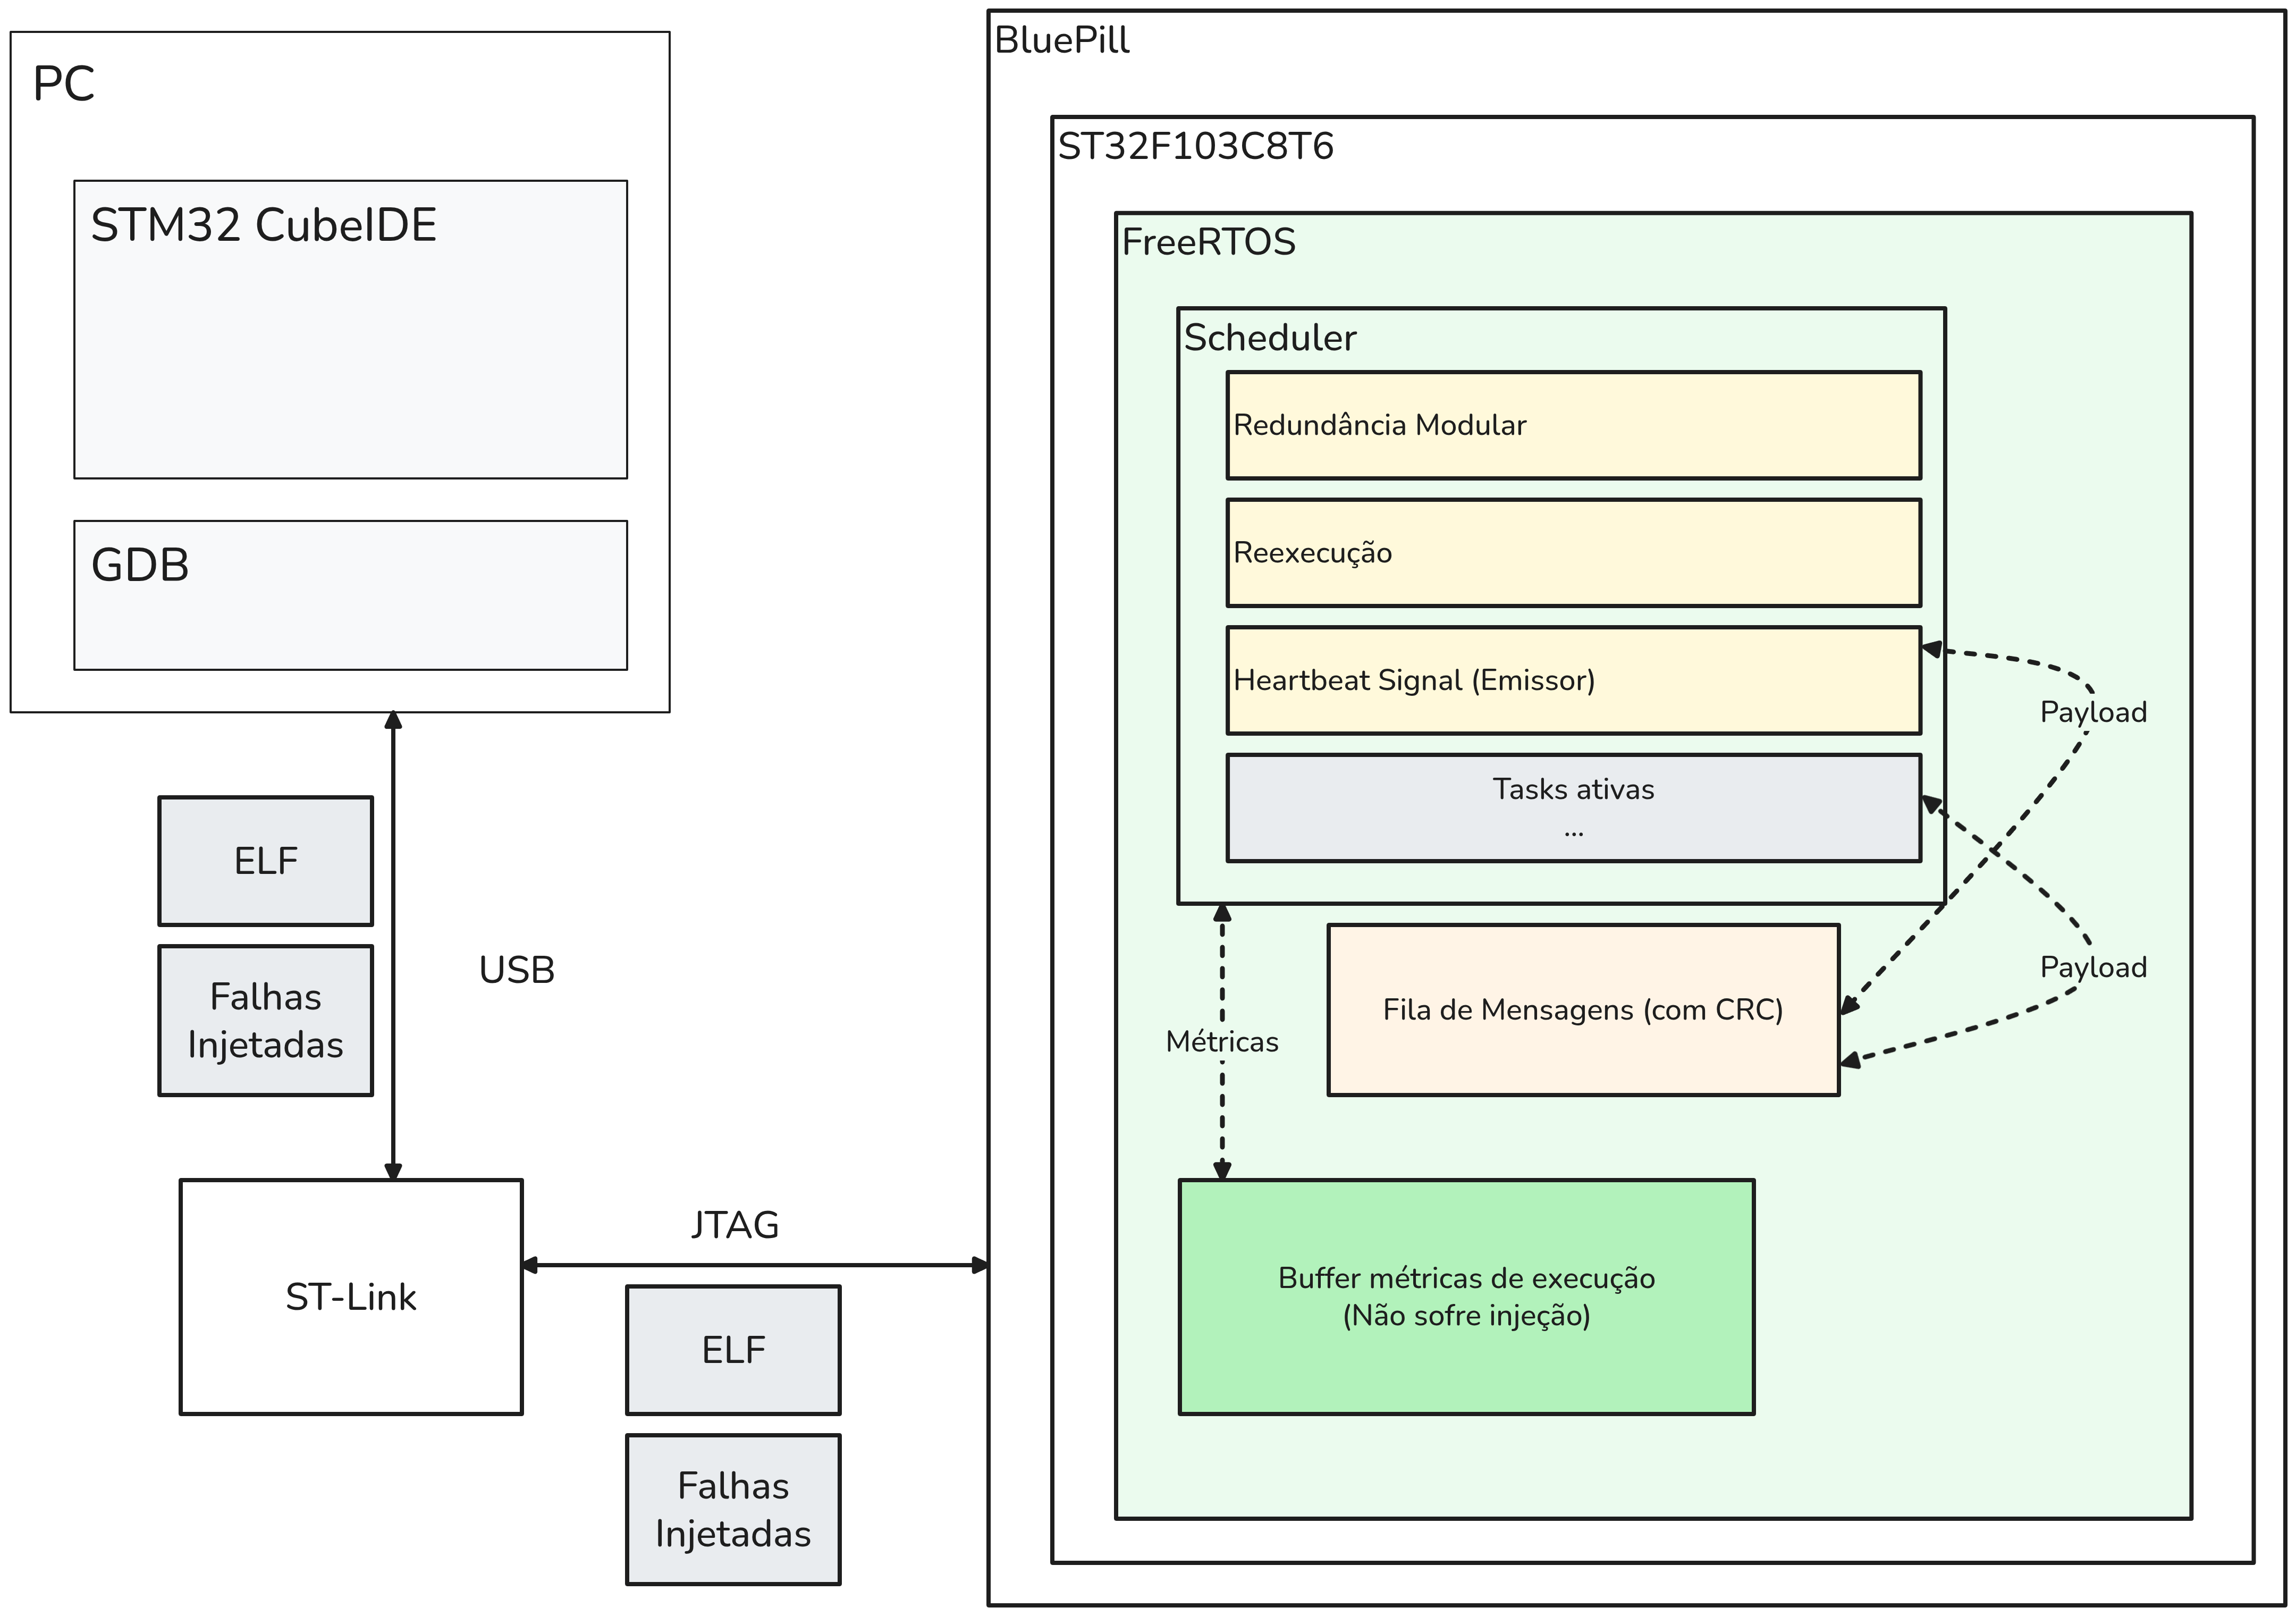
\includegraphics[width=0.97\textwidth]{assets/visao_geral.png}
    \captionsetup{justification=raggedright}
    \caption*{Fonte: Elaborada pelo autor}
    \label{fig:visaoGeral}
\end{figure}

\section{Premissas}

% TODO: Termos em ingles
Será partido do ponto que ao menos o processador que executa o escalonador terá registradores de controle (ponteiro de pilha, contador de programa, endereço de retorno) que sejam capazes de mascarar falhas. Apesar de ser possível executar os algoritmos reforçados com análise de fluxo do programa e adicionar redundância aos registradores, isso adiciona um grau a mais de complexidade que foge do escopo do trabalho. Como mencionado na \autoref{sec:trabRel}, a memória fora do banco de registradores pode ser duas ordens de magnitude mais sensível à eventos disruptivos \cite{ReliabilityArmCortexUnderHeavyIons}.

Com o fim de reduzir o tamanho do executável e manter o fluxo de mais previsível não serão utilizados mecanismos de exceção com desenrolamento (\textit{unwinding}) da pilha. Também não será utilizado de RTTI (Runtime Type Information). Todos os erros devem portanto ser tratados como valores ou como falhas lógicas.

Necessariamente, é preciso também presumir que testes sintéticos possam ao menos aproximar a performance do mundo real, ou ao menos prever o pior caso possível com grau razoável de acurácia. O uso de testes sintéticos não deve ser um substituto para a medição em uma aplicação real, porém, uma bateria de testes com injeção artificial de falhas pode ser utilizada para verificar as tendências e custos relativos introduzidos, mesmo que não necessariamente reflitam as medidas absolutas do produto final.

Portanto, será assumido que os resultados extraídos de injeção de falhas artificiais, apesar de menos condizentes com os valores absolutos de uma aplicação e não sendo substitutos adequados na fase de aprovação de um produto real, são ao menos capazes para realizar uma análise quanto ao custo proporcional introduzido, e devido à sua facilidade de realização e profundidade de inspeção possível, serão priorizados inicialmente neste projeto.

\section{Metodologia}

\subsection{Materiais}

% TODO: sumarizar, mais diagramas, melhorar coesao deixar um pouco mais segmentado e com conexoes entre os topicos, aqui e em metodos. referenciar as figuras

Será utilizada a linguagem C++ com o compilador GCC (ou Clang), o alvo principal do trabalho será um microcontrolador STM32F103C8T6 "Bluepill" 32-bits da arquitetura ARMv7-M, como visto na \autoref{fig:stm32Bluepill}.

\begin{figure}[H]
    \centering
    \captionsetup{justification=centering}
    \caption{Diagrama da STM32F103C8T6 ("Bluepill")}
    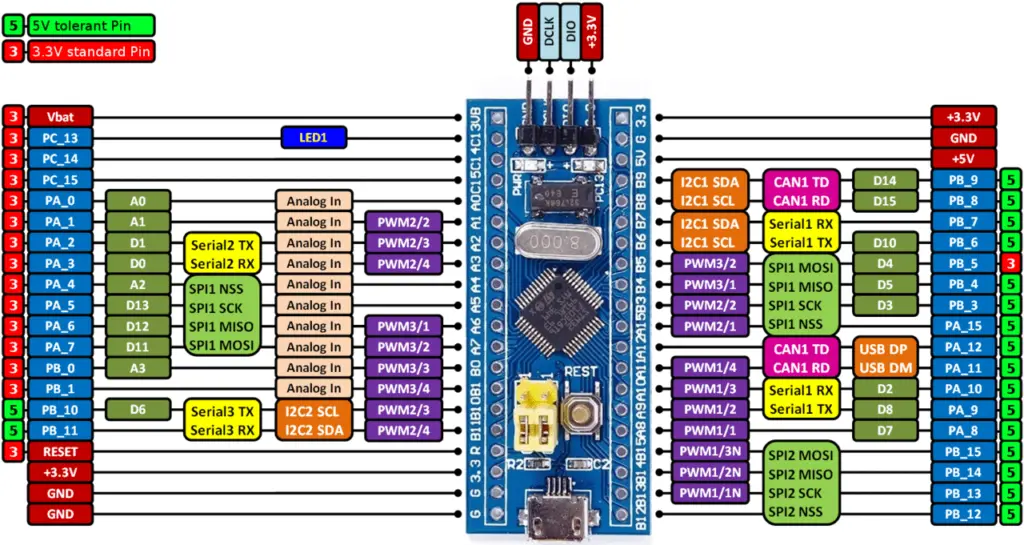
\includegraphics[width=0.80\textwidth]{assets/stm32_bluepill.png}
    \captionsetup{justification=raggedright}
    \caption*{Fonte: \figcite{STMBoardProductPage}}
    \label{fig:stm32Bluepill}
\end{figure}

Para a injeção de falhas será utilizado o depurador GDB em conjunto com uma ferramenta de depuração de hardware ST-LINK (\autoref{fig:stLink}), a comunicação do ST-LINK é feita via USB com o computador e via JTAG com o microcontrolador alvo, também será usado em conjunto uma IDE fornecida pelo mesmo fabricante, a STM32Cube IDE.

\begin{figure}[H]
    \centering
    \captionsetup{justification=centering}
    \caption{ST-LINK/V2}
    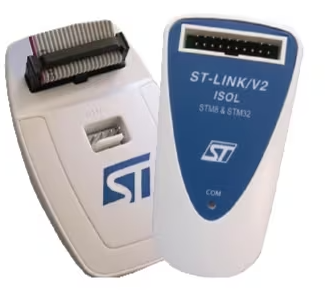
\includegraphics[width=0.50\textwidth]{assets/st_link.png}
    \captionsetup{justification=raggedright}
    \caption*{Fonte: \figcite{STLinkProductPage}}
    \label{fig:stLink}
\end{figure}

\begin{figure}[H]
    \centering
    \captionsetup{justification=centering}
    \caption{ST-LINK/V2}
    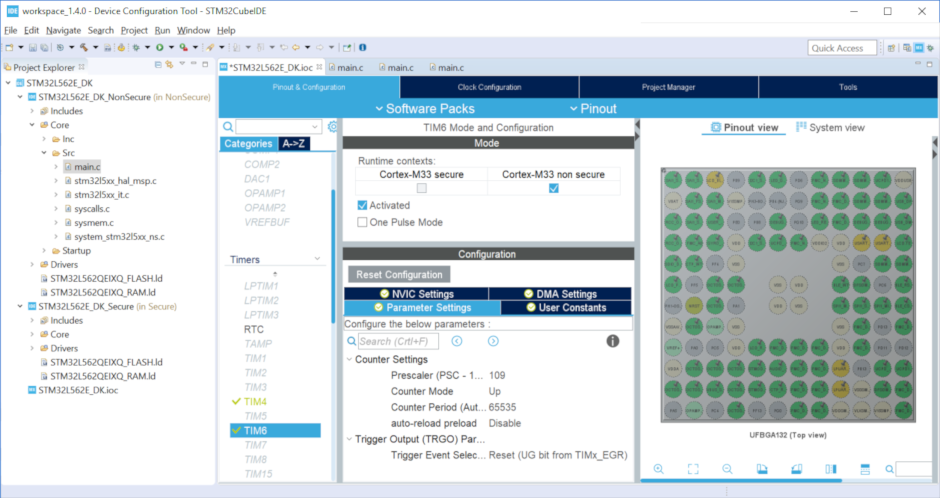
\includegraphics[width=0.80\textwidth]{assets/stmcube_ide.png}
    \captionsetup{justification=raggedright}
    \caption*{Fonte: \figcite{STMCubeProductPage}}
    \label{fig:stmCubeIDE}
\end{figure}

% #sourced_image(
%   caption: [STMCube IDE],
%   source: "STMCubeProductPage",
%   image("assets/stmcube_ide.png"))

Durante a fase de desenvolvimento dos algoritmos será utilizado o QEMU juntamente com as ferramentas anteriormente citadas, assim como sanitizadores de memória e condições de corrida (ASan, TSan, UBSan) para auxiliar na detecção de erros mais cedo durante o desenvolvimento.

O sistema operacional de tempo real escolhido foi o FreeRTOS, por ser extensivamente testado e documentado e prover um escalonador totalmente preemptivo com um custo espacial relativamente pequeno, além disso, os contribuidores do FreeRTOS mantém uma lista grande de versões para diferentes arquiteturas e controladores, facilitando drasticamente o trabalho ao não ter que criar uma HAL do zero.

\subsection{Métodos}

Serão utilizadas as seguintes técnicas de tolerância à falhas implementadas em software: CRCs para mensagens, redundância modular, reexecução, sinal heartbeat e asserts. O detalhamento específico de cada técnica é abordado em maior detalhe na \autoref{subsec:algoritmos}.

Para a criação da análise, serão realizados testes com injeção lógica em hardware utilizando-se do ST-Link em combinação com um computador que emitirá os comandos para injeção via depurador, as falhas serão de natureza transiente e afetarão valores na memória (corrupção silenciosa) assim como nos registradores que não são de controle. A \autoref{fig:injecaoHardwareLogica} detalha de forma mais específica o fluxo de gerar uma falha. As combinações específicas de falhas e técnicas escolhidas são abordadas na \autoref{subsec:campanhaInjecao}.

% TODO: Diagrama
%\begin{figure}[H]
%    \centering
%    \captionsetup{justification=centering}
%    \caption{Injeção lógica em hardware}
%    \includegraphics[width=0.90\textwidth]{assets/injecao_logica_hardware.png}
%    \captionsetup{justification=raggedright}
%   \caption*{Fonte: Elaborada pelo autor}
%    \label{fig:injecaoHardwareLogica}
%\end{figure}


A coleta de métricas será realizada com os mecanismos de monitoramento do sistema FreeRTOS juntamente com contadores de incremento atômico, o tempo de execução das tarefas, seu espaço de memória utilizado e o número de falhas detectadas será armazenado em uma estrutura que residirá em um segmento de memória que é deliberadamente isento de falhas.

Com o objetivo de promover a reutilização de código e a abstração, será implementada uma interface que generaliza um objeto de tarefa. Considerando que um objeto que realiza despache dinâmico requer uma tabela de despacho virtual (V-Table), faz-se necessário adotar precauções adicionais, dado que a própria tabela pode estar sujeita a falhas. Para mitigar esse risco, será aplicada uma replicação simples dos ponteiros de função da V-Table, resultando em um custo adicional de duas comparações por chamada de método. A interação da interface com o resto do sistema é abordada em maior detalhe na \autoref{subsec:interface}.

\section{Análise de requisitos}
\label{sec:req}

\begin{quadro}[H]
    \centering
    \caption{Requisitos funcionais}
    \begin{tabular}{|p{0.125\textwidth}|p{0.8\textwidth}|}
        \hline
        \rowcolor[HTML]{C0C0C0}
        \textbf{Requisito} & \textbf{Descrição}  \\
        \hline
        
        \textbf{RF01} & Implementação de todos os algoritmos descritos na \autoref{subsec:algoritmos} \\ 
        \hline

        \textbf{RF02} & Criação, finalização e cancelamento de tarefas e recuperação de sua memória alocada \\
        \hline
        
        \textbf{RF03} & Configuração do mecanismo de tolerância, prioridade e prazo de execução da tarefa \\
        \hline

        \textbf{RF04} & Cumprimento do prazo estipulado no momento de criação da tarefa caso não exista presença de falhas \\
        \hline

        \textbf{RF05} & Detecção e reação à falhas de corrupção de memória \\
        \hline

        \textbf{RF06} & Detecção e reação à falhas de vencimento de prazo de execução \\
        \hline
        
        \textbf{RF07} & Monitoramento do número de falhas detectadas e violações de prazos  \\
        \hline
        
        \textbf{RF08} & Comunicação entre tarefas por uma fila com checagem dos pacotes \\
        \hline
        
    \end{tabular}
    \label{tab:rf}
\end{quadro}

\begin{quadro}[H]
    \centering
    \caption{Requisitos não funcionais}
    \begin{tabular}{|p{0.125\textwidth}|p{0.8\textwidth}|}
        \hline
        \rowcolor[HTML]{C0C0C0}
        \textbf{Requisito} & \textbf{Descrição}  \\
        \hline
        
        \textbf{RNF01} & Em caso de falha catastrófica (sem possibilidade de tolerância) o sistema deve ser capaz de reiniciar  \\ 
        \hline

        \textbf{RNF02} & O consumo de memória deve ser pré determinado em tempo de compilação ou na inicialização do sistema \\
        \hline
        
        \textbf{RNF03} & A interface deve estar acima do escalonador preemptivo do FreeRTOS \\
        \hline

        \textbf{RNF04} & Deve ser compatível com arquitetura ARMv7M ou ARMv8M \\
        \hline

        \textbf{RNF05} & Implementação realizada em C++ (versão 20 ou acima) \\
        \hline
        
        \textbf{RNF06} & Código fonte da interface disponível sob licença permissiva (BSD3) \\
        \hline

    \end{tabular}
    \label{tab:rnf}
\end{quadro}

\subsection{Interface} \label{subsec:interface}

Para melhor generalizar o uso das técnicas, utiliza-se de uma abstração da estrutura de tarefa para facilitar a utilização de diferentes técnicas de execução sem necessitar de alterações significativas por parte do usuário da interface.

Uma mensagem envelopa um pacote de dados qualquer para que possa ser enviado de forma assíncrona entre tarefas. Neste caso, o ordenamento dos campos é importante: o pacote precisa ser o último membro para serialização de estruturas de tamanho arbitrário, a distribuição dos campos na memória é demonstrada na \autoref{fig:messageStruct}. 

\begin{figure}[H]
    \centering
    \captionsetup{justification=centering}
    \caption{Layout de uma mensagem}
    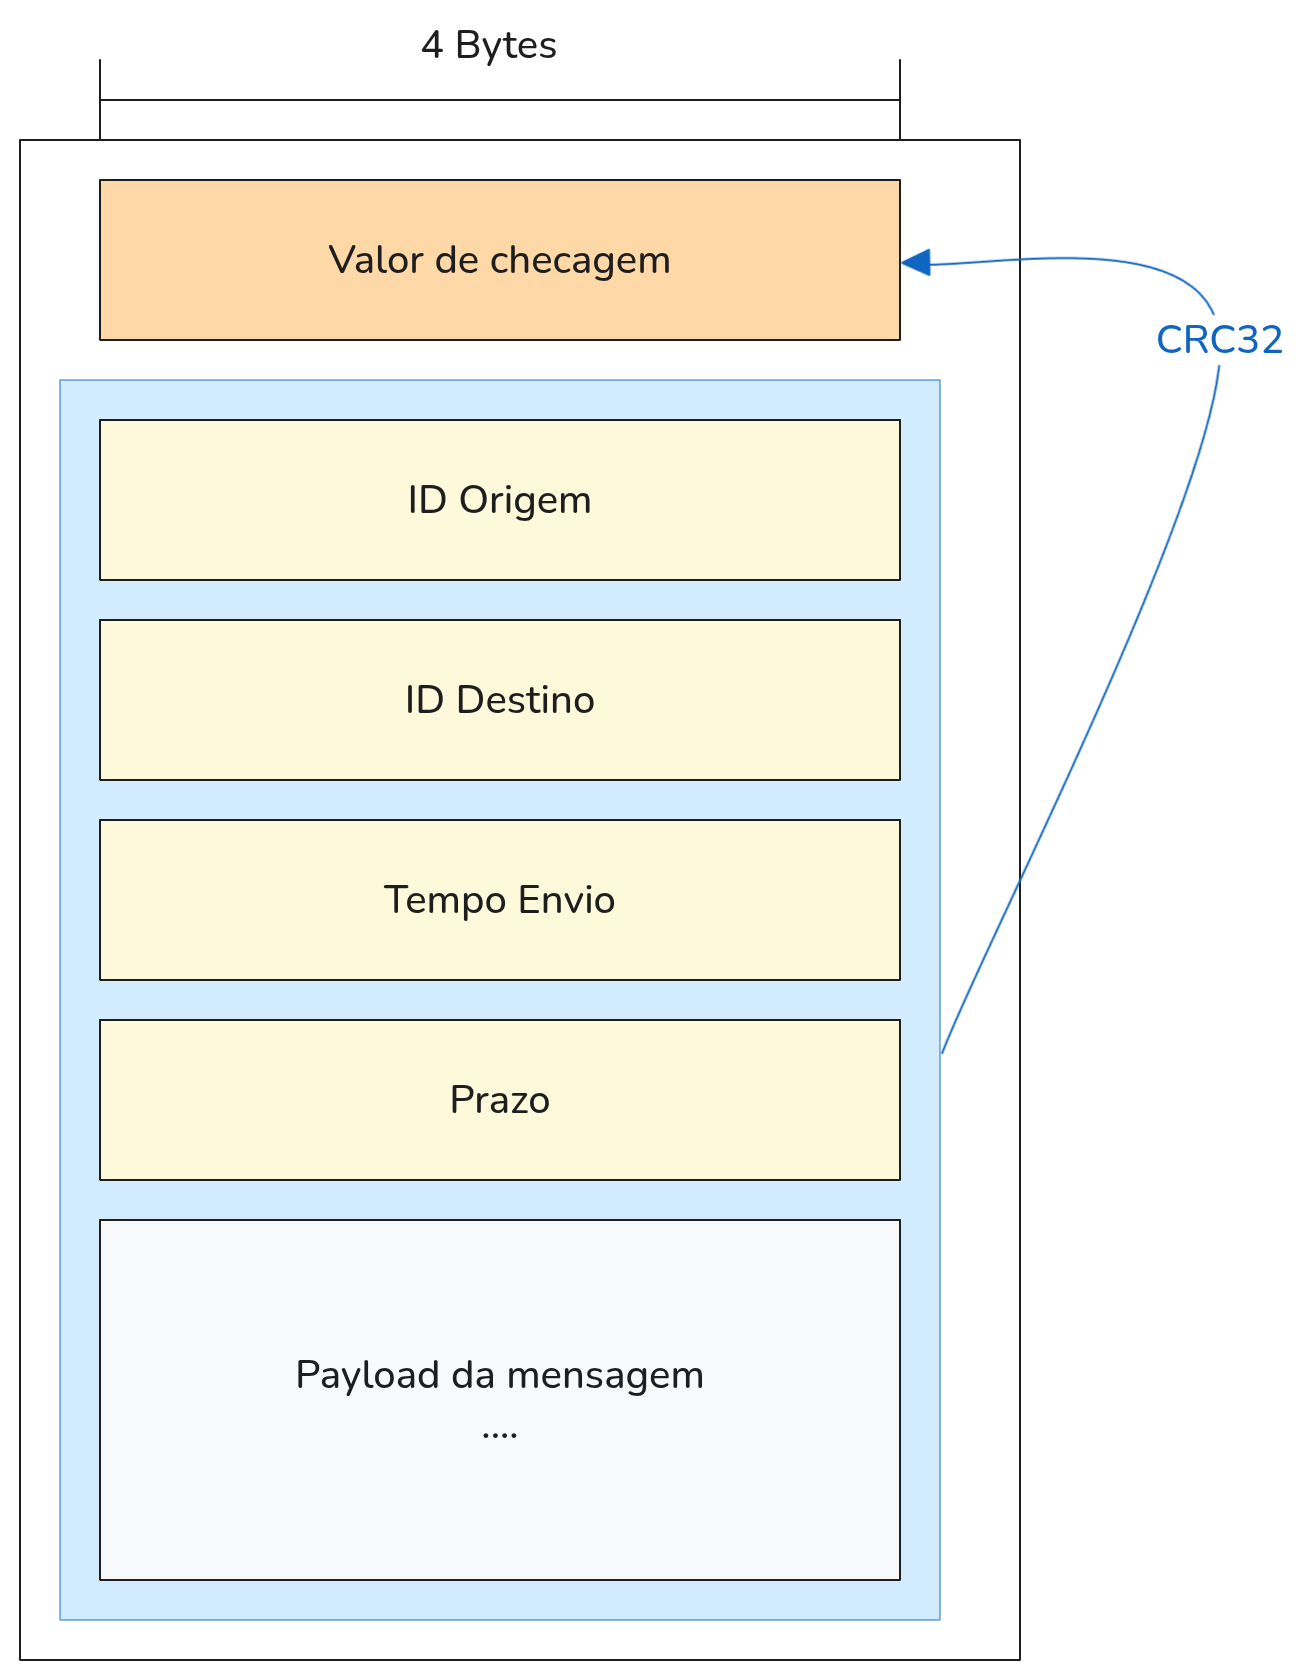
\includegraphics[width=0.60\textwidth]{assets/payload_layout.png}
    \captionsetup{justification=raggedright}
    \caption*{Fonte: Elaborada pelo autor}
    \label{fig:messageStruct}
\end{figure}

A tarefa é um objeto de interface que abstrai parte do estado utilizado pelo RTOS e provê métodos para sua inicialização, término e cancelamento. Uma tarefa possui um espaço de pilha dedicado, e uma V-Table que inclui os métodos providos para sua execução. A identificação da tarefa se dá pelo seu ID, que diretamente mapeia o recurso que encapsula o estado da tarefa no RTOS. O diagrama na \autoref{fig:bddTarefa} demonstra a relação de uma tarefa e os outros componentes do sistema.

\begin{figure}[H]
    \centering
    \captionsetup{justification=centering}
    \caption{Objeto que implementa a interface de Tarefa}
    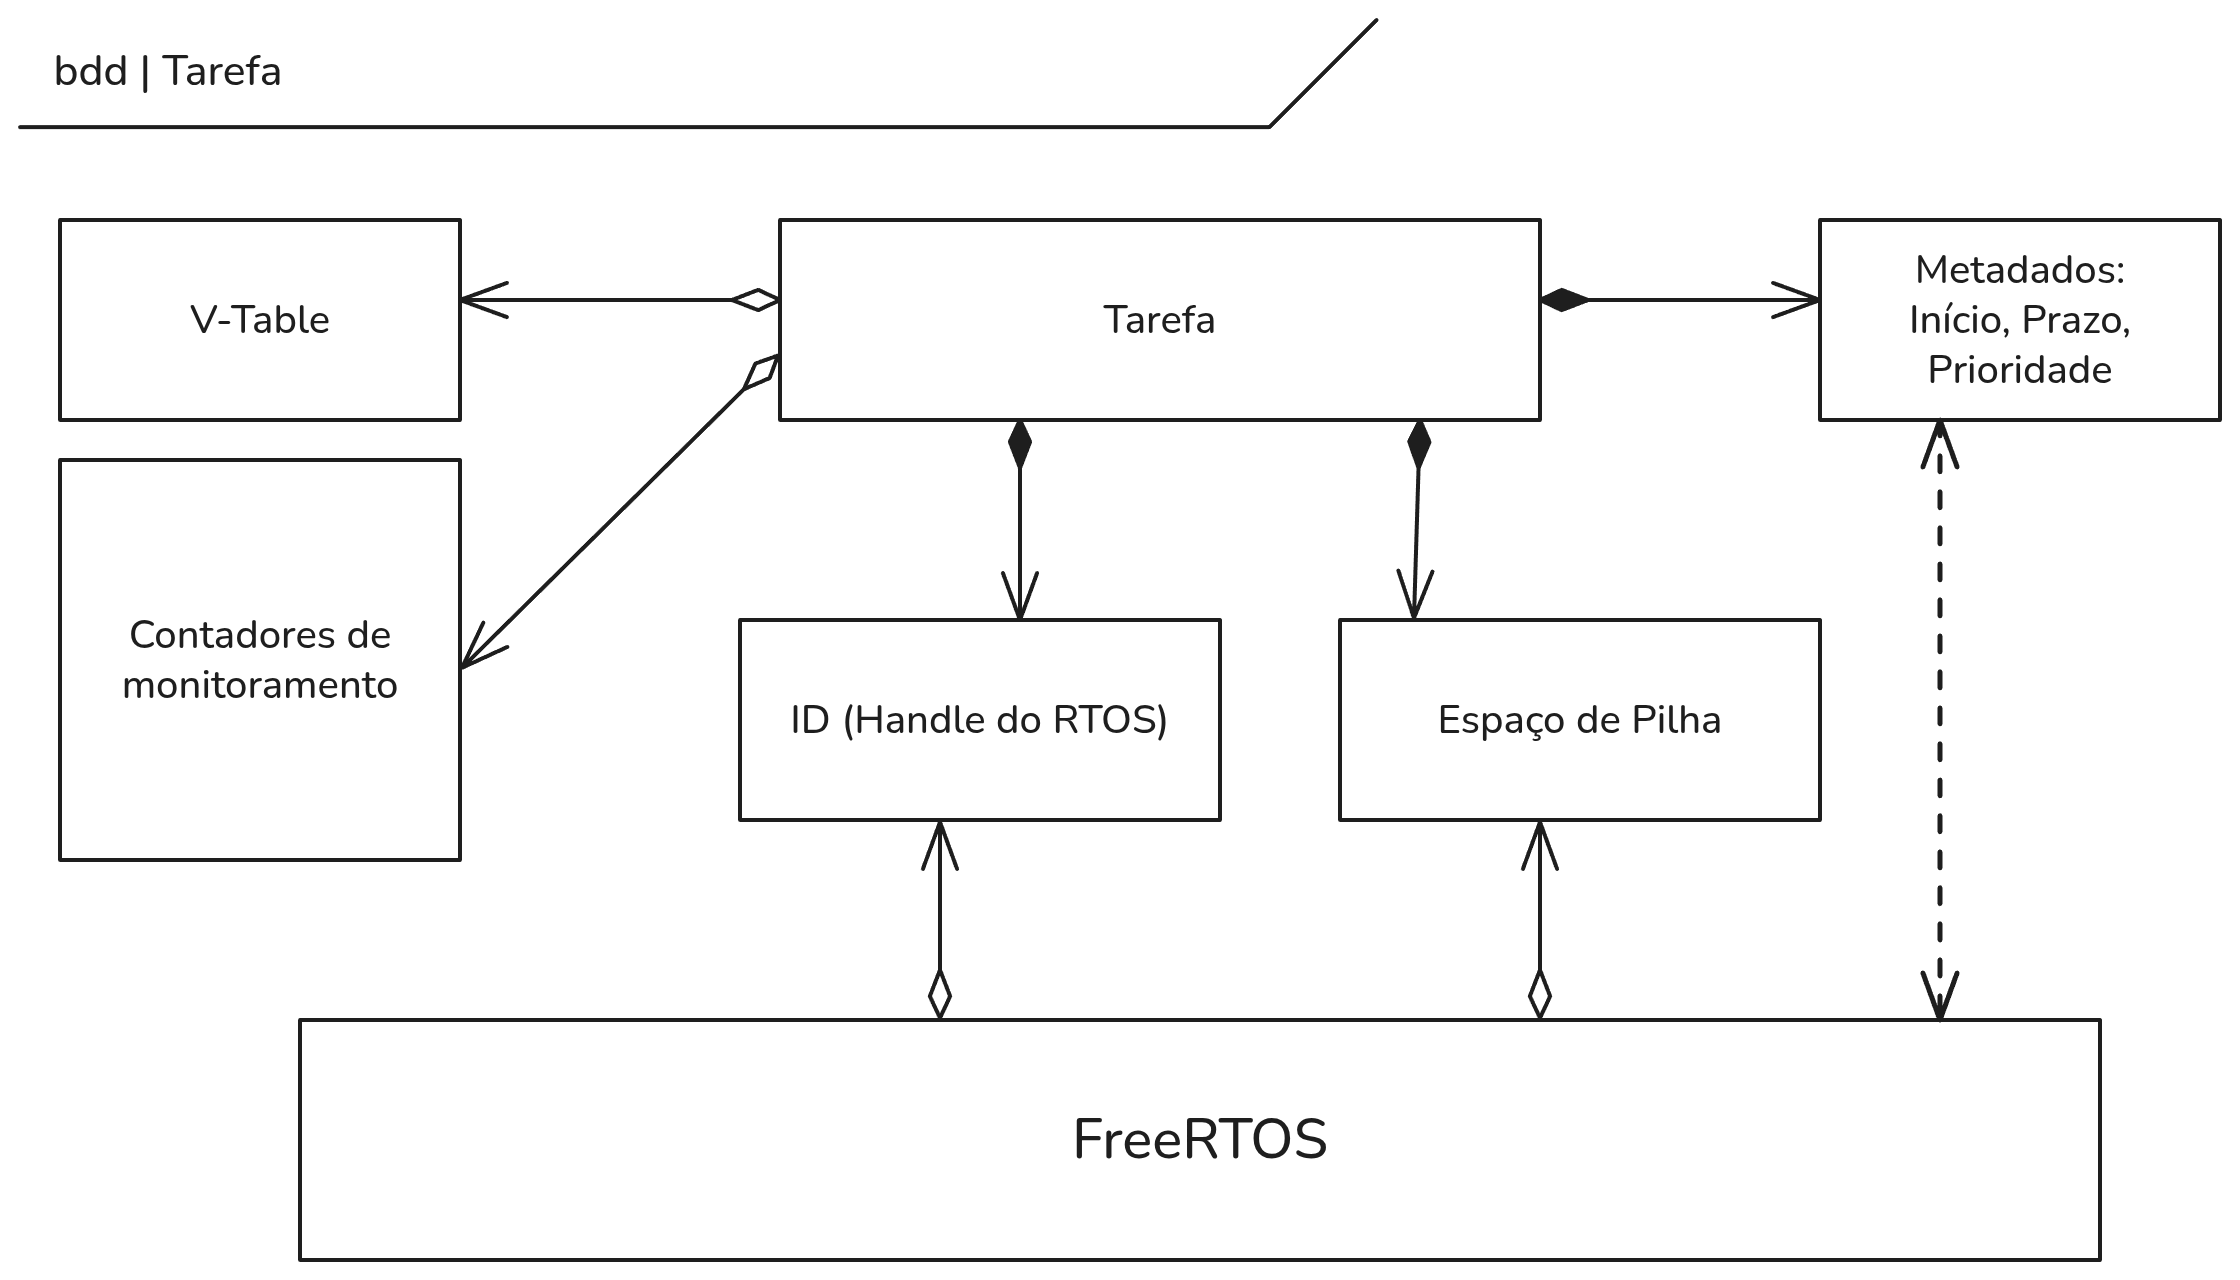
\includegraphics[width=0.90\textwidth]{assets/task_bdd.png}
    \captionsetup{justification=raggedright}
    \caption*{Fonte: Elaborada pelo autor}
    \label{fig:bddTarefa}
\end{figure}

A \autoref{fig:bddTarefa} omite a replicação da V-Table por clareza visual, mas antes da invocação de qualquer método da V-Table, será feito uma comparação adicional com outras duas tabelas redundantes para detectar corrupções na própria tabela durante a indireção por ponteiro de função.

\subsection{Algoritmos e Técnicas} \label{subsec:algoritmos}

Para a implementação da funcionalidade de tolerância à falhas, algumas das técnicas abordadas no \autoref{cap:fund} serão utilizadas. O detalhamento sobre a implementação será abordado nesta seção.

\subsubsection{CRC: Cyclic Redundancy Check}
% TODO fazer!

\subsubsection{Redundância Modular}

Para a aplicação da redundância modular, neste caso a redundância modular tripla, será feito a replicação concorrente da tarefa, cada tarefa possui um espaço de pilha próprio e são escalonadas de forma convencional pelo FreeRTOS. O corpo das tarefas não é replicado, e continua como parte de memória para apenas leitura e execução, um exemplo da relação de réplicas de tarefas executando em relação ao resto do sistema pode ser observado na \autoref{fig:bddTMR}.

\begin{figure}[H]
    \centering
    \captionsetup{justification=centering}
    \caption{Diagrama de bloco de Redundância modular}
    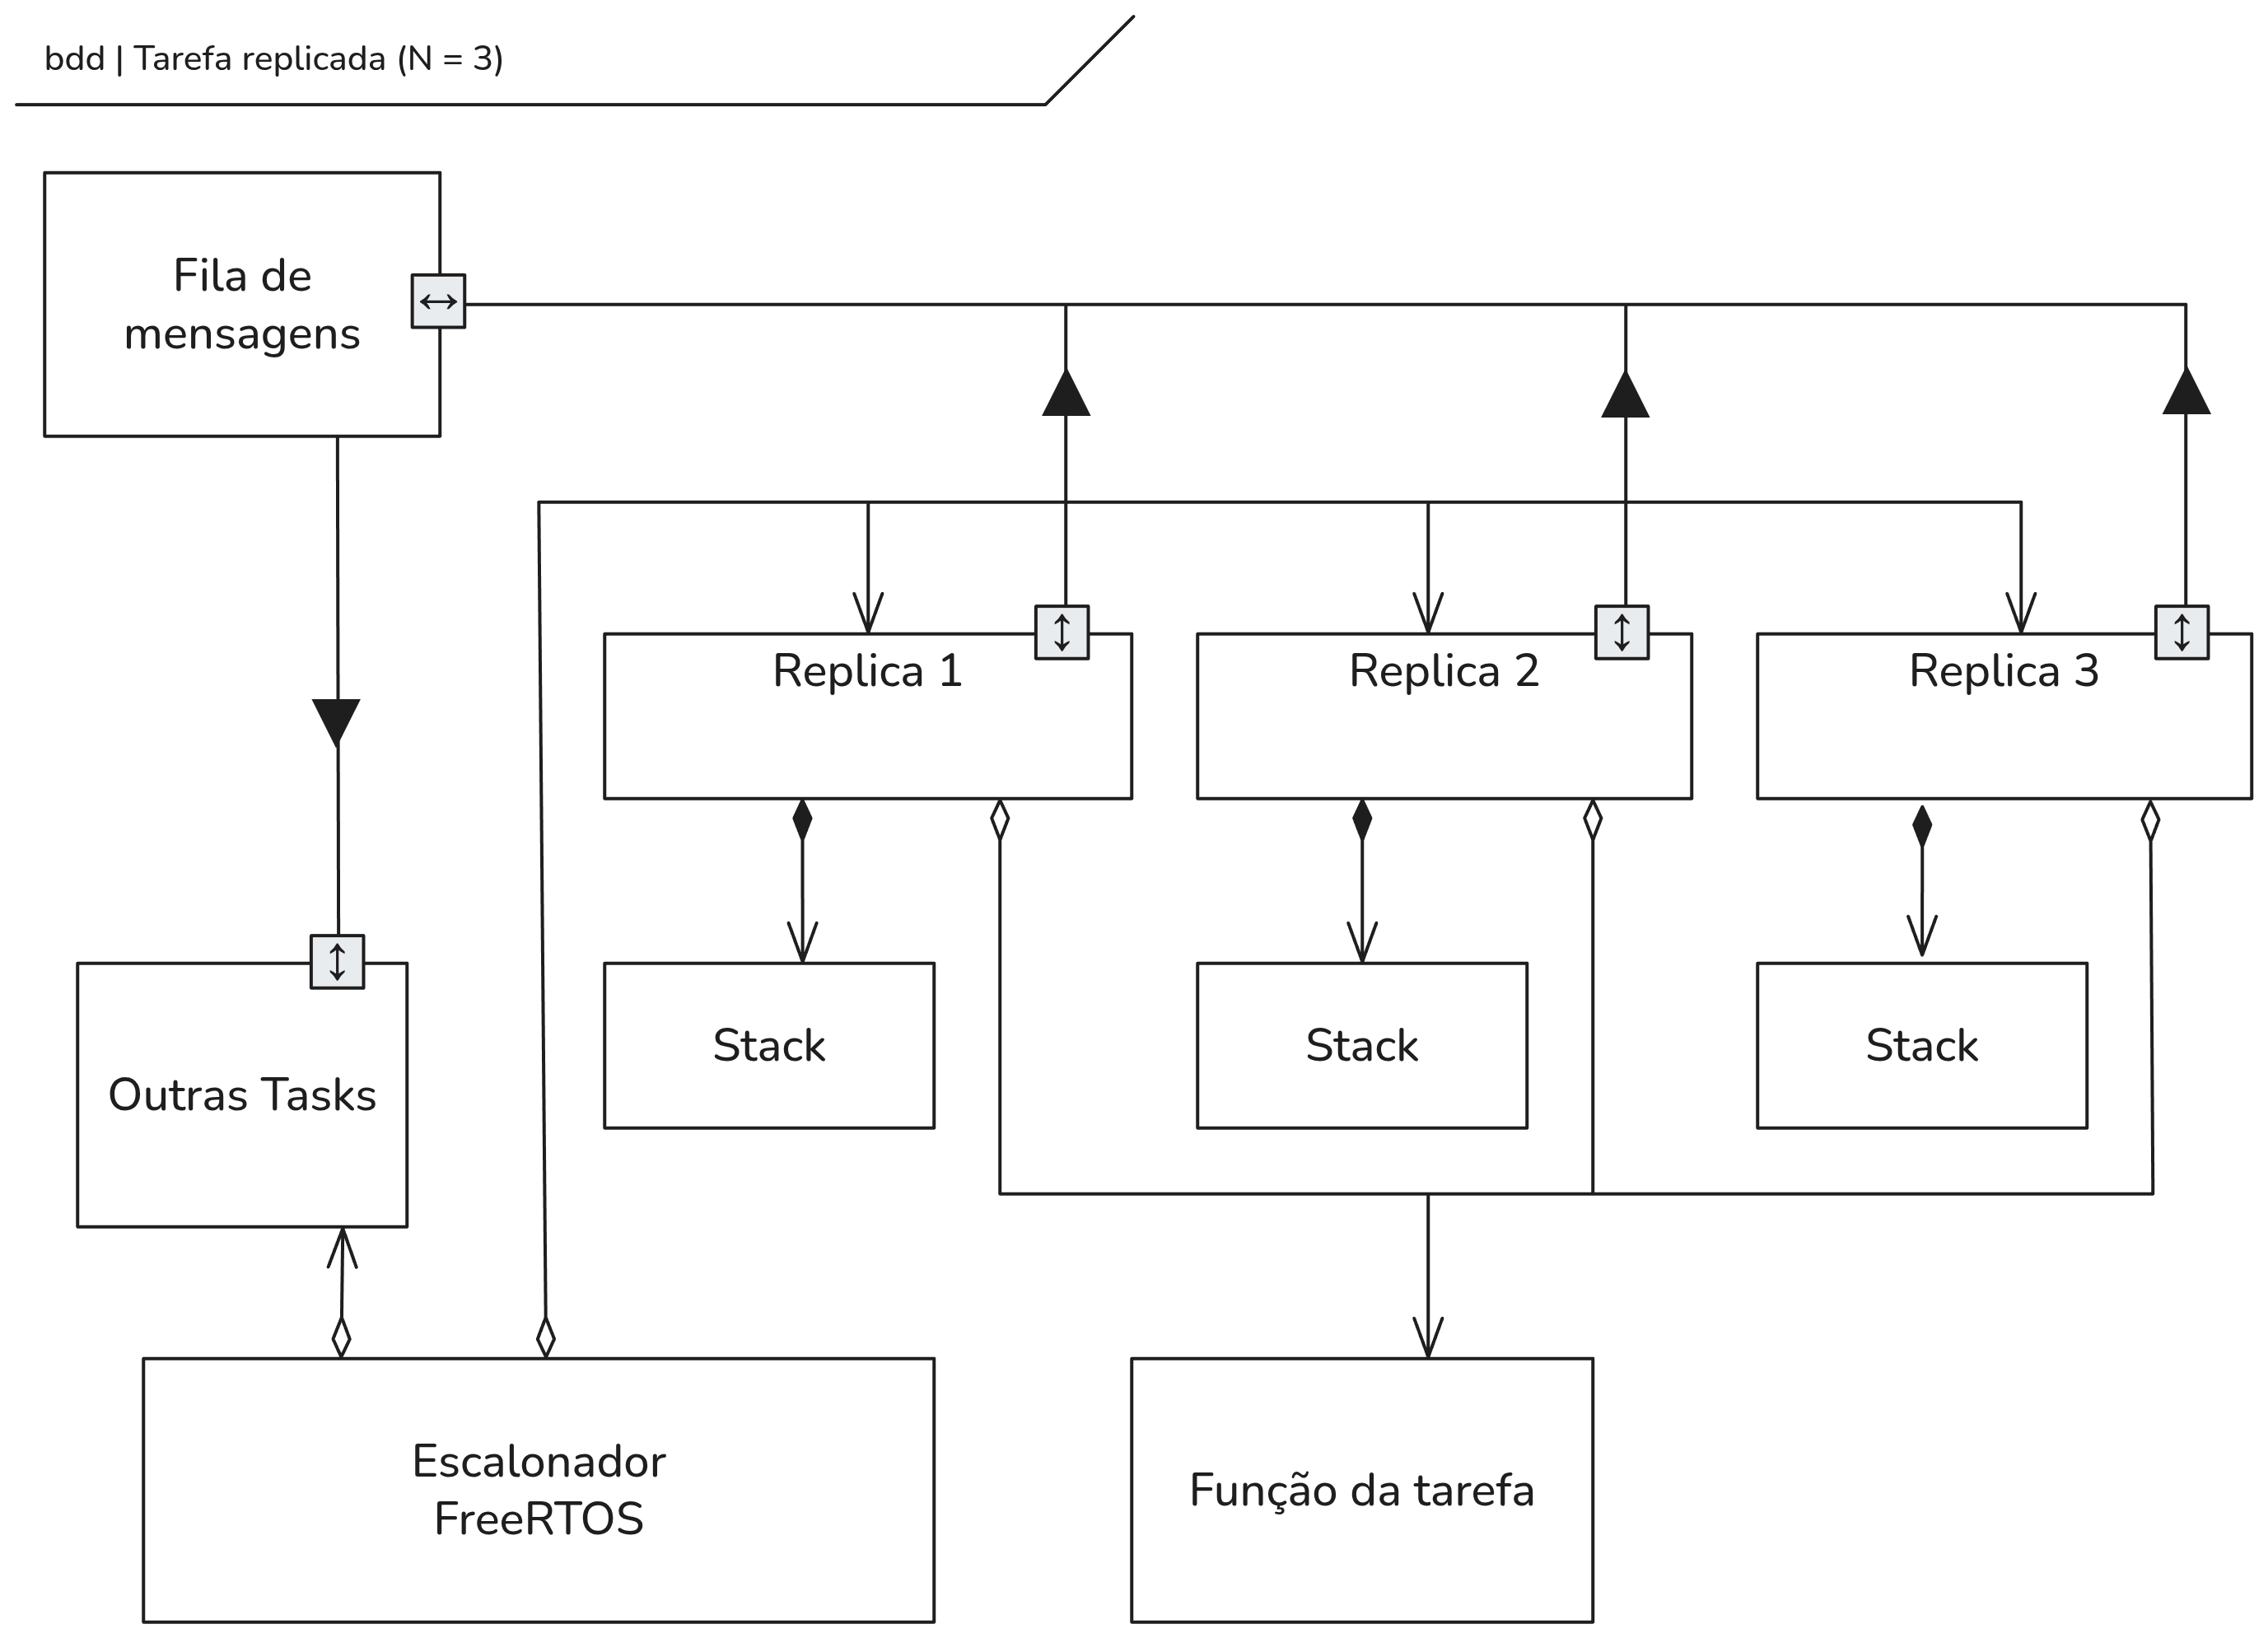
\includegraphics[width=0.975\textwidth]{assets/tmr_bdd.png}
    \captionsetup{justification=raggedright}
    \caption*{Fonte: Elaborada pelo autor}
    \label{fig:bddTMR}
\end{figure}

\subsubsection{Reexecução}
% TODO disagrama

\subsubsection{Heartbeat Signal}
\subsubsection{Asserts}

\section{Plano de Verificação}
\subsection{Campanha de Injeção de Falhas} \label{subsec:campanhaInjecao}

% 02/07
% Associar coisas do plano de verificação aos requisitos
% Falar de tempo real no visão geral
% 03/07
% Refazer consideracoes finais
% 04/07
% Ler o trabalho da Nicole
% COlocar como trabalho relacionado no lugar do de analise de fluxo la

% \begin{quadro}[H]
%     \centering
%     \noindent
%     \caption{Requisitos não funcionais}
%     \begin{tabular}{|p{0.15\textwidth}|p{0.8\textwidth}|}
%         \hline
%         \rowcolor[HTML]{C0C0C0}
%         \textbf{Requisito} & \textbf{Descrição}  \\
%         \hline
%         \textbf{RNF01} & O algoritmo de CNN deve ser treinado em Python com as bibliotecas TensorFlow, Keras e scikit-learn\\
%         \hline
%         \textbf{RNF02} & A CNN embarcada deverá ser desenvolvida usando as bibliotecas TensorFlow Lite e/ou TinyML\\
%         \hline
%         \textbf{RNF03} & O algoritmo de CNN deve ser implementado em linguagem C para ser embarcado\\
%         \hline
%         \textbf{RNF04} & O algoritmo de CNN deve ser embarcado no microcontrolador ESP32 e/ou Raspberry Pi Pico\\
%         \hline
%         \textbf{RNF05} & A memória consumida pelo algoritmo não deve ser maior que 4 MB\\
%         \hline
%         \textbf{RNF06} & A CNN embarcada deve ser implementada usando ESP-IDF para ESP32\\
%         \hline
%         \textbf{RNF07} & A CNN embarcada deve ser implementada usando Pico C/C++ SDK\\
%         \hline
%     \end{tabular}
%     \label{tab:rnf}
% \end{quadro}

 \clearpage
\chapter{Considerações Finais}
\label{cap:consid}

Durante a pesquisa bibliográfica, foi possível observar uma variedade de técnicas de tolerância à falhas em software. Das técnicas escolhidas, optou-se por focar em técnicas mais simples para a detecção (CRC e asserts) e técnicas de execução que possibilitem a criação de condições de transparência.

O projeto de pesquisa visa avaliar a aplicação destas técnicas em um contexto de um sistema operacional de tempo real, utilizando de injeção de falhas lógicas em hardware para a construção de uma análise do impacto de diferentes combinações de técnicas. Algumas das hipóteses levantadas foram:

\begin{itemize}
    \item[1] Asserts terão um impacto pequeno na performance.
    \item[2] Replicação de tarefas introduzirá maior variância no tempo de execução.
    \item[3] Reexecução terá uma variância menor do que a replicação, porém com maior custo de tempo.
    \item[4] Sinais de heartbeat terão um impacto menor na detecção de erros em relação à outras técnicas.
\end{itemize}

 \clearpage
% TCC 3
% \input{4_desenvolvimento} \clearpage
% \input{5_resultados} \clearpage
% \input{6_consideracoes} \clearpage

\postextual
\bibliography{refs.bib}  \clearpage
%\input{anexo/0_anexo.tex} \clearpage

\end{document}
